\clearpage
\subsection{Model inspection: 0-lepton channel}
\label{sec:fit_0lep}
We show the results for the model inspection and discuss the goodness of the fit model for the \zlep channel in this section.
In contrast to the combined (0,1,2-lepton channel) fit, in the 0-lepton-only fit it is not possible to constrain the \Wjets and \Zjets \ backgrounds individually.
In the combined fit the former can be constrained by the 1-lepton and the latter by the 2-lepton channel.
In the 0-lepton channel however both backgrounds have similar yields and shapes.
As a consequence the floating normalizations for these backgrounds are combined into a single \Vjets normalization (which is split in two by resolved/merged regime).
A similar approach was chosen for the systematic \Wjets/\Zjets \ modelling uncertainty which here is implemented with a single nuisance parameter for \Vjets.
No other norm apart from \Vjets is left floating.
Instead $t\bar t$ and single top norms are implemented with a $30\%$ prior and the diboson norm with a $40\%$ prior.
These numbers are based on the difference in pre-fit event yields of $t\bar t$ and diboson background when simulated with nominal and alternative MC samples shown in Tab. \ref{fig:fit_0lep_priors}.

\begin{figure}[ht]
\begin{tabular}{r|c|c|c|c|c}
 $t\bar t$ yields& merged SR HP  & merged SR LP & resolved SR & merged CR & resolved CR\\
 \hline
 nominal &1533 &2009 &1284 &4361 &21802\\
 alternative &1064 &1678 &941 &3997 &16184\\
 (nom-alt)/nom &31$\%$ &16$\%$ &27$\%$ &8$\%$ &26$\%$\\
\end{tabular}
$ $\\
\begin{tabular}{r|c|c|c|c|c}
 diboson yields& merged SR HP  & merged SR LP & resolved SR & merged CR & resolved CR\\
 \hline
 nominal &208 &275 &586 &494 &4376\\
 alternative &142 &164 &512 &260 &2652\\
 (nom-alt)/nom &32$\%$ &40$\%$ &13$\%$ &47$\%$ &39$\%$\\
\end{tabular}
\caption{Difference in pre-fit event yields of the $t\bar t$ and diboson background when simulated with nominal and alternative MC samples.}
\label{fig:fit_0lep_priors}
\end{figure}

\clearpage
\subsubsection{Prefit plots}
Figure \ref{fig:fit_0lep_prefit} shows the pre-fit plots of the analysis regions entering in the \zlep fit only model; 
in particular, \mjjtag distributions in \Wjets/\Zjets CRs are shown and the neural network scores distributions  are shown in the SRs, only the left side bins are plotted using real data as well.
\begin{figure}[ht]
      \centering
	\subfigure[Merged HP SR 0lep]{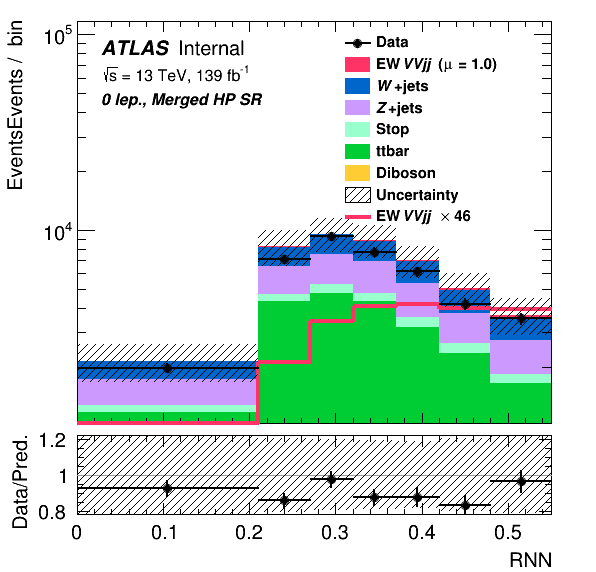
\includegraphics[width=0.32\textwidth]{figures/0lep/fit/left/Region_distRNN_DSRVBSHP_BMin0_J0_incJet1_L0_T0_incFat1_Y6051_incTag1_Fat1_Prefitlog}}
	\subfigure[Merged LP SR 0lep]{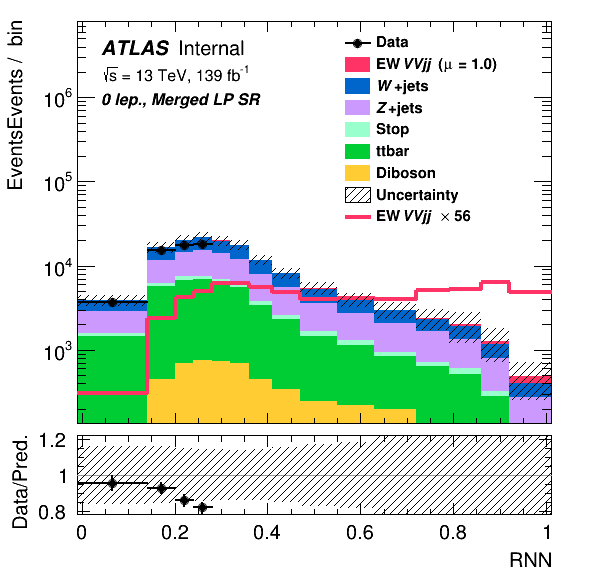
\includegraphics[width=0.32\textwidth]{figures/0lep/fit/left/Region_distRNN_DSRVBSLP_BMin0_J0_incJet1_L0_T0_incFat1_Y6051_incTag1_Fat1_Prefitlog}}
	\subfigure[Resolved SR 0lep]{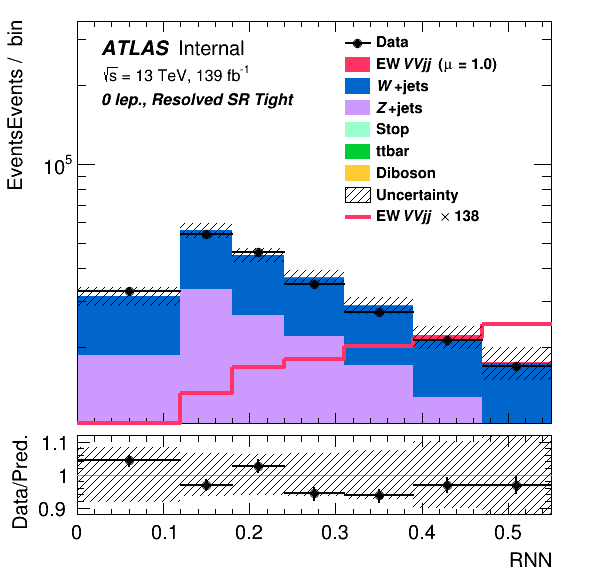
\includegraphics[width=0.32\textwidth]{figures/0lep/fit/left/Region_distRNN_DSRVBSTight_BMin0_T0_Y6051_incTag1_J2_L0_incJet1_Prefitlog}}
\\
	\subfigure[Merged VjetCR 0lep]{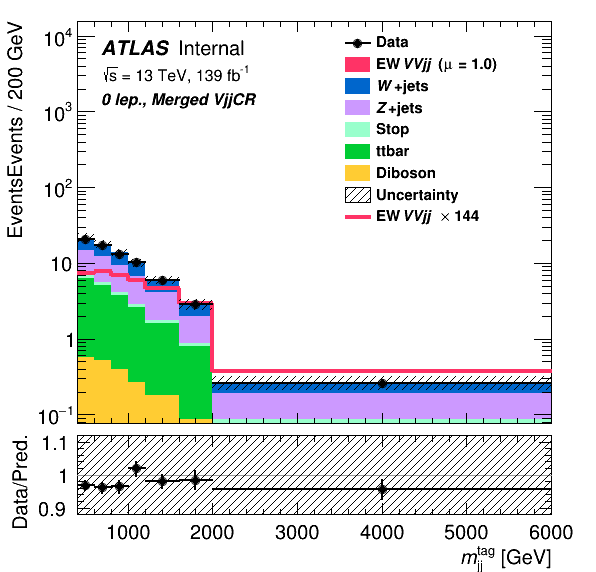
\includegraphics[width=0.32\textwidth]{figures/0lep/fit//left/Region_disttagMjj_DCRVjetMerged_BMin0_J0_incJet1_L0_T0_incFat1_Y6051_incTag1_Fat1_Prefitlog}}
	\subfigure[Resolved VjetCR 0lep]{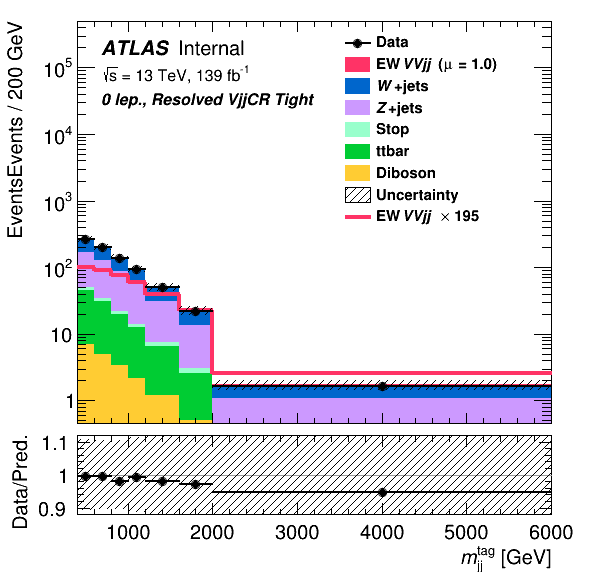
\includegraphics[width=0.32\textwidth]{figures/0lep/fit/left/Region_disttagMjj_DCRVjetTight_BMin0_T0_Y6051_incTag1_J2_L0_incJet1_Prefitlog}}
\\
	\caption{Prefit plots for the 0 lepton channel. Data is blinded in the right bins that contain 75\% signal. [The x-axis is wrong, only unblinded bins are shown.]}
       \label{fig:fit_0lep_prefit}
\end{figure}

\clearpage
\subsubsection{Prefit tables}
Table \ref{tab:fit_0lep_prefit_yields} shows the expected yields for signal and background processes in all the control and signal regions for the \zlep channel.

%\begin{figure}[ht]
%      \centering
%	\subfigure[Merged HP SR 0lep]{\begin{tabular}{l|c|}
\cline{2-2}
 & \multicolumn{1}{c|}{merged HP SR}\\
W & 777.52 $\pm$ 105.08\\
Z & 848.97 $\pm$ 116.99\\
Diboson & 207.59 $\pm$ 89.22\\
stop & 189.68 $\pm$ 65.46\\
ttbar & 1533.32 $\pm$ 551.71\\
\hline
Bkg & 3557.08 $\pm$ 673.74\\
\hline
Signal & 92.23 $\pm$ 12.68\\
\end{tabular}
}
%	\subfigure[Merged LP SR 0lep]{\begin{tabular}{l|c|}
\cline{2-2}
 & \multicolumn{1}{c|}{merged LP SR}\\
W & 2123.99 $\pm$ 201.96\\
Z & 2568.04 $\pm$ 247.79\\
Diboson & 274.60 $\pm$ 115.66\\
stop & 230.32 $\pm$ 74.22\\
ttbar & 2009.29 $\pm$ 648.94\\
\hline
Bkg & 7206.25 $\pm$ 907.32\\
\hline
Signal & 73.40 $\pm$ 10.60\\
\end{tabular}
}
%	\subfigure[Resolved SR 0lep]{\begin{tabular}{l|c|}
\cline{2-2}
 & \multicolumn{1}{c|}{resolved SR}\\
W & 8756.32 $\pm$ 598.11\\
Z & 10859.56 $\pm$ 722.80\\
Diboson & 586.01 $\pm$ 235.93\\
stop & 329.14 $\pm$ 100.11\\
ttbar & 1283.59 $\pm$ 388.36\\
\hline
Bkg & 21814.63 $\pm$ 1436.58\\
\hline
Signal & 217.99 $\pm$ 19.03\\
\end{tabular}
}
%\\
%	\subfigure[Merged VjetCR 0lep]{\begin{tabular}{l|c|}
\cline{2-2}
 & \multicolumn{1}{c|}{merged CR}\\
W & 5395.71 $\pm$ 497.99\\
Z & 6493.33 $\pm$ 608.23\\
Diboson & 494.25 $\pm$ 201.86\\
stop & 467.34 $\pm$ 148.16\\
ttbar & 4361.00 $\pm$ 1434.51\\
\hline
Bkg & 17211.62 $\pm$ 2034.79\\
\hline
Signal & 70.06 $\pm$ 8.90\\
\hline
Data & 16833 \\
\end{tabular}
}
%	\subfigure[Resolved VjetCR 0lep]{\begin{tabular}{l|c|}
\cline{2-2}
 & \multicolumn{1}{c|}{resolved CR}\\
W & 67436.46 $\pm$ 7029.01\\
Z & 80524.07 $\pm$ 8571.96\\
Diboson & 4375.68 $\pm$ 1772.51\\
stop & 3463.97 $\pm$ 1066.33\\
ttbar & 21802.09 $\pm$ 6725.53\\
\hline
Bkg & 177602.28 $\pm$ 18817.47\\
\hline
Signal & 515.46 $\pm$ 38.31\\
\hline
Data & 175982 \\
\end{tabular}
}
%\\
%	\caption{Prefit yields for the 0 lepton channel.}
%       \label{fig:fit_0lep_prefit_yields}
%\end{figure}

\begin{table}
%\begin{center}
\centering
%\small
%\scalebox{0.60}{
\begin{tabular}{l|c|}
\cline{2-2}
% & \multicolumn{1}{c|}{Region\_distMTagMerJets\_DCRVjet\_BMin0\_J0\_incJet1\_L2\_T0\_incFat1\_Y6051\_incTag1\_Fat1}\\
 & \multicolumn{1}{c|}{\tlep - ZCR Merged} \\
%\cline{2-2}
% & \multicolumn{1}{c|}{Region\_distMTagMerJets\_DCRVjet\_BMin0\_J0\_incJet1\_L2\_T0\_incFat1\_Y6051\_incTag1\_Fat1}\\ 
\hline
W & 3.13 $\pm$ 0.35\\
Z & 7964.27 $\pm$ 792.98\\
Diboson & 283.38 $\pm$ 143.63\\
stop & 8.21 $\pm$ 2.92\\
ttbar & 194.44 $\pm$ 28.20\\
\hline
Bkg & 8453.43 $\pm$ 844.02\\
\hline
EW6llqq & 29.67 $\pm$ 3.73\\
\hline
Signal & 29.67 $\pm$ 3.73\\
SignalExpected & 29.67 $\pm$ 3.73\\
\hline
S/B & 3.51e-03\\
S/sqrt(S+B) & 3.22e-01\\
\hline
data & 6645\\ \hline
\end{tabular}
%}
%\end{table}
%\begin{table}
%\centering
%\small
%\scalebox{0.60}{
\begin{tabular}{l|c|}
\cline{2-2}
% & \multicolumn{1}{c|}{Region\_distMTagResJets\_DCRVjetFid\_BMin0\_T0\_Y6051\_incTag1\_J2\_L2\_incJet1}\\
 & \multicolumn{1}{c|}{\tlep - ZCR Resolved}\\
%\cline{2-2}
% & \multicolumn{1}{c|}{Region\_distMTagResJets\_DCRVjetFid\_BMin0\_T0\_Y6051\_incTag1\_J2\_L2\_incJet1}\\ 
\hline
W & 57.63 $\pm$ 11.31\\
Z & 228206.01 $\pm$ 39622.91\\
Diboson & 4645.71 $\pm$ 1460.84\\
stop & 266.54 $\pm$ 88.88\\
ttbar & 7306.82 $\pm$ 1070.92\\
\hline
Bkg & 240482.70 $\pm$ 40883.23\\
\hline
EW6llqq & 421.60 $\pm$ 31.07\\
\hline
Signal & 421.60 $\pm$ 31.07\\
SignalExpected & 421.60 $\pm$ 31.07\\
\hline
S/B & 1.75e-03\\
S/sqrt(S+B) & 8.59e-01\\
\hline
data & 200097\\ \hline
\end{tabular}
%}
%\end{table}
%\begin{table}
%\centering
%\small
%\scalebox{0.60}{
\begin{tabular}{l|c|}
\cline{2-2}
% & \multicolumn{1}{c|}{Region\_distRNNScoreMerged\_DSRVBSHP\_BMin0\_J0\_incJet1\_L2\_T0\_incFat1\_Y6051\_incTag1\_Fat1}\\
 & \multicolumn{1}{c|}{\tlep - SR Merged HP}\\
%\cline{2-2}
% & \multicolumn{1}{c|}{Region\_distRNNScoreMerged\_DSRVBSHP\_BMin0\_J0\_incJet1\_L2\_T0\_incFat1\_Y6051\_incTag1\_Fat1}\\ 
\hline
W & 0.61 $\pm$ 0.09\\
Z & 1082.40 $\pm$ 136.78\\
Diboson & 109.07 $\pm$ 56.98\\
stop & 2.28 $\pm$ 0.78\\
ttbar & 31.77 $\pm$ 5.25\\
\hline
Bkg & 1226.12 $\pm$ 157.65\\
\hline
EW6llqq & 36.75 $\pm$ 6.68\\
\hline
Signal & 36.75 $\pm$ 6.68\\
SignalExpected & 36.75 $\pm$ 6.68\\
\hline
S/B & 3.00e-02\\
S/sqrt(S+B) & 1.03e+00\\
\end{tabular}
%}
%\end{table}
%\begin{table}
%\centering
%\small
%\scalebox{0.60}{
\begin{tabular}{l|c|}
\cline{2-2}
% & \multicolumn{1}{c|}{Region\_distRNNScoreMerged\_DSRVBSLP\_BMin0\_J0\_incJet1\_L2\_T0\_incFat1\_Y6051\_incTag1\_Fat1}\\
 & \multicolumn{1}{c|}{\tlep - SR Merged LP}\\
%\cline{2-2}
% & \multicolumn{1}{c|}{Region\_distRNNScoreMerged\_DSRVBSLP\_BMin0\_J0\_incJet1\_L2\_T0\_incFat1\_Y6051\_incTag1\_Fat1}\\ 
\hline
W & 1.73 $\pm$ 0.25\\
Z & 3158.10 $\pm$ 272.60\\
Diboson & 147.28 $\pm$ 75.88\\
stop & 3.82 $\pm$ 1.28\\
ttbar & 75.10 $\pm$ 9.62\\
\hline
Bkg & 3386.03 $\pm$ 297.69\\
\hline
EW6llqq & 29.70 $\pm$ 5.57\\
\hline
Signal & 29.70 $\pm$ 5.57\\
SignalExpected & 29.70 $\pm$ 5.57\\
\hline
S/B & 8.77e-03\\
S/sqrt(S+B) & 5.08e-01\\
\end{tabular}
%}
%\end{table}
%\begin{table}
%\centering
%\small
%\scalebox{0.60}{
\begin{tabular}{l|c|}
\cline{2-2}
% & \multicolumn{1}{c|}{Region\_distRNNScoreResolved\_DSRVBSFid\_BMin0\_T0\_Y6051\_incTag1\_J2\_L2\_incJet1}\\
 & \multicolumn{1}{c|}{\tlep - SR Resolved}\\
%\cline{2-2}
% & \multicolumn{1}{c|}{Region\_distRNNScoreResolved\_DSRVBSFid\_BMin0\_T0\_Y6051\_incTag1\_J2\_L2\_incJet1}\\ 
\hline
W & 14.10 $\pm$ 2.80\\
Z & 31415.55 $\pm$ 3624.61\\
Diboson & 599.57 $\pm$ 183.15\\
stop & 31.03 $\pm$ 9.66\\
ttbar & 819.35 $\pm$ 90.79\\
\hline
Bkg & 32879.61 $\pm$ 3693.20\\
\hline
EW6llqq & 175.42 $\pm$ 12.15\\
\hline
Signal & 175.42 $\pm$ 12.15\\
SignalExpected & 175.42 $\pm$ 12.15\\
\hline
S/B & 5.34e-03\\
S/sqrt(S+B) & 9.65e-01\\
\end{tabular}
%}
%\end{center}
\caption{Prefit event yields for the analysis regions in the 2 lepton channel.}
\label{tab:2lepPrefitYield}
\end{table}
%%% Local Variables:
%%% mode: latex
%%% TeX-master: "../../../../ANA-STDM-2018-27-INT1"
%%% End:




\clearpage
\subsubsection{Asimov Fit Results}
A fit to the full range of SRs using Asimov data is performed only with \zlep channel.
Figures \ref{fig:fit_0lep_fcc_asimov}, \ref{fig:fit_0lep_corr_asimov}, and \ref{fig:fit_0lep_ranking_asimov} show the pulls, the correlation and the ranking respectively of the NPs used in the fit.
\begin{figure}[ht]
      \centering
        \includegraphics[width=\linewidth]{figures/0lep/fit/full/NP_allExceptGammas.pdf}
        \caption{Fit cross-check, conditional fit ($\mu=1$) to asimov data in the full range for the 0 lepton channel only.}
       \label{fig:fit_0lep_fcc_asimov}
\end{figure}
\begin{figure}[ht]
      \centering
        \includegraphics[width=\linewidth]{figures/0lep/fit_SMApp/SemileptonicVBS_mc16ade_v2.RNN_ResBoo_0lep_SemileptonicVBS_13TeV_Systs_FS0_0_RNN_ResBoo_0lep/plots/fcc/AsimovFit_unconditionnal_mu1/corr_HighCorrNoMCStat.pdf}
        \caption{Correlations for unconditional fit ($\mu=1$) to asimov data in the full range for the 0 lepton channel only.}
       \label{fig:fit_0lep_corr_asimov}
\end{figure}
\begin{figure}[ht]
      \centering
        \includegraphics[width=0.6\textwidth]{figures/StatisticalInterpretation/new_rankings/Ranking_postfit_0lep}
        \caption{Ranking plot for unconditional fit ($\mu=1$) to asimov data in the full range, for the 0 lepton channel only.}
       \label{fig:fit_0lep_ranking_asimov}
\end{figure}

Regarding the pull plot just shown and all the ones shown in the following, 
we can give more details about the black boxes that are shown.
For a given NP, such a box gives an approximate measure of the compatibility of the fitted pull 
with the associated postfit constraint. 
A small pull almost unconstrained is less likely than a large pull with a tight constraint. 
The good reference is Nicolas Morange's habilitation thesis, which can be found at \cite{morange:tel-03341303};
the general concept is explained at pages 58-59, more specifically bottom of page 58 and top of page 59, 
and more details are given in A1 p109+.

In particular, we found a few parameters that are constrained in the fit; they are:

\begin{itemize}
      \item \texttt{SysMJJREWEIGHT\_100per} (L0\_Fat1 for merged and L0\_J2 for resolved) 
            are the \mjjtag reweighting uncertainties for merged and resolved regions;
            We expected these constraints since we take the \mjjtag reweighting as 100\% uncertainties 
            and we, indeed, let the control regions to constrain these systematic uncertainties.

      \item \texttt{SysMODEL\_V\_MGPy8} is the shape difference between Sherpa samples 
      (after the \mjjtag reweighting applied) 
      and the MadGraph samples (no \mjjtag reweighting applied).
      The analysis is, indeed, affected by this uncertainty 
      since the well-known modelling difference between the two generators is related 
      to the high \mjjtag and jets multiplicity phase space; 

      \item \texttt{SysFATJET\_BJT\_JET\_JetTagSF\_Hadronisation} is the hadronisation model uncertainty 
      provided by the central CP recommendations; the impact on the fitted mu is very low, indeed, it is low ranked
      and it does not appear on the top of the ranking plot \ref{fig:fit_0lep_ranking_asimov}.

      \item \texttt{Normttbar0Lep} is the normalisation for the ttbar process; there is no specific top CR 
      in the \zlep channel fit; it will be better handled in the combined leptons channel fit.

      \item \texttt{SysMODEL\_ttbar\_PwHwg7} is the modelling uncertainty for the ttbar process 
      coming from the alternative Powheg/Herwig sample; the impact on the fitted $\mu$ 
      is about $5\%$ (Figure \ref{fig:fit_0lep_ranking_asimov}).

\end{itemize}

Furthermore, the leading uncertainty impacting on the fitted $\mu$ ($\sim 10\%$) 
are found to be the Theory QCD on the signal and the modeling uncertainty of the \Vjets;
also, the normalisation of the \ttbar is highly ranked but this will be better constrained
in the combined fit using the dedicated \olep TopCR.

\clearpage
\subsubsection{Left Bins Data Fit Results}
According to the unblinding strategy, the fit model is inspected in the left side of our SRs using data fit; 
the goal is to spot some problematics pulls that might appear in the final data fit.

Figures \ref{fig:fit_0lep_fcc_left} and \ref{fig:fit_0lep_corr_left} show the pulls and the correlations respectively of the NPs used in the fit.
\begin{figure}[ht]
      \centering
        \includegraphics[width=\linewidth]{figures/0lep/fit/left/NP_allExceptGammas.pdf}
        \caption{Fit cross-check, unconditional fit ($\mu=1$) to data in the left bins only, for the 0 lepton channel only.}
       \label{fig:fit_0lep_fcc_left}
\end{figure}
\begin{figure}[ht]
      \centering
        \includegraphics[width=\linewidth]{figures/0lep/fit_SMApp/SemileptonicVBS_mc16ade_v2.RNN_ResBoo_0lep_leftOnly_SemileptonicVBS_13TeV_Systs_FS0_0_RNN_ResBoo_0lep_leftOnly/plots/fcc/GlobalFit_unconditionnal_mu1/corr_HighCorrNoMCStat.pdf}
        \caption{Correlations for unconditional fit ($\mu=1$) to data in the left bins only, for the 0 lepton channel only.}
       \label{fig:fit_0lep_corr_left}
\end{figure}

The \zlep only fit looks quite healthy;
similar constraints are found in the left bins only fit as well, 
they have been already discussed in the Asimov fit results. 
In addition, the observed pulls are all contained inside the 1 sigma band; 
the two NPs that are worth to mention from the pulls check are:

\begin{itemize}
      \item \texttt{SysJET\_Flavor\_Response}, it is the Flavor Response uncertainties for small-R jets, 
      introduced in section \ref{subsec:bkg_uncer_qg}.

      \item \texttt{SysQG\_exp}, it is an experimental uncertainty about tracks multiplicity modelling
      coming from data measurements, as discussed in section \ref{subsec:tracks_uncer}.

\end{itemize}

both of them will be better discussed in the combined fit section \ref{sec:fit_combo},
but they already look low ranked in the \zlep channel fit, Figure \ref{fig:fit_0lep_ranking_asimov}.
